% ============================================================================
% CAPÍTULO 2 — REFERENCIAL TEÓRICO
% ============================================================================

\chapter{Referencial Teórico}
\label{cap:referencial}

O presente capítulo reúne os fundamentos conceituais necessários para compreender a proposta metodológica deste trabalho. São abordados, inicialmente, os princípios da montagem \textit{de novo} de genomas e as especificidades do DNA mitocondrial, que justificam sua relevância como objeto de estudo. Em seguida, discute-se a questão da reprodutibilidade em ciência computacional e as soluções contemporâneas oferecidas pela engenharia de software, com destaque para a tecnologia de conteinerização. Por fim, apresentam-se os sistemas de gerenciamento de workflows científicos, cuja integração com containers constitui a base para a construção de pipelines modernos, portáveis e reprodutíveis.

\section{Montagem \textit{De Novo} de Genomas e a Análise Mitocondrial}

Em bioinformática, a \textbf{montagem de genomas} (\textit{genome assembly}) consiste no processo computacional de reconstruir a sequência original de DNA a partir de fragmentos obtidos por tecnologias de Sequenciamento de Nova Geração (NGS). O conceito é análogo à reconstrução de um texto completo a partir de milhões de trechos sobrepostos --- cada trecho sendo uma \textbf{leitura} (\textit{read}), um fragmento curto de sequência gerado pelo sequenciador. O método mais amplamente utilizado para gerar esses fragmentos é o \textit{shotgun sequencing}, no qual o DNA genômico é clivado aleatoriamente em milhões de pequenos pedaços que, posteriormente, são sequenciados. Essa estratégia garante alta \textbf{cobertura} do genoma --- isto é, cada posição do DNA é representada por múltiplas leituras, tipicamente dezenas a centenas de vezes ---, mas resulta em dados fragmentados que precisam ser cuidadosamente alinhados e sobrepostos para permitir a reconstrução da sequência completa \cite{ekblom2014}. A complexidade computacional dessa tarefa motivou o desenvolvimento de algoritmos especializados, baseados em técnicas como grafos de De Bruijn --- estrutura em que cada nó representa uma subsequência de $k$ nucleótidos consecutivos (denominada \textbf{k-mer}), e cada aresta representa sobreposições entre k-mers adjacentes --- e estratégias de sobreposição-layout-consenso \cite{miller2010}.

% [SUGESTÃO DE FIGURA]: Diagrama ilustrativo do processo de shotgun sequencing
\begin{figure}[H]
    \centering
    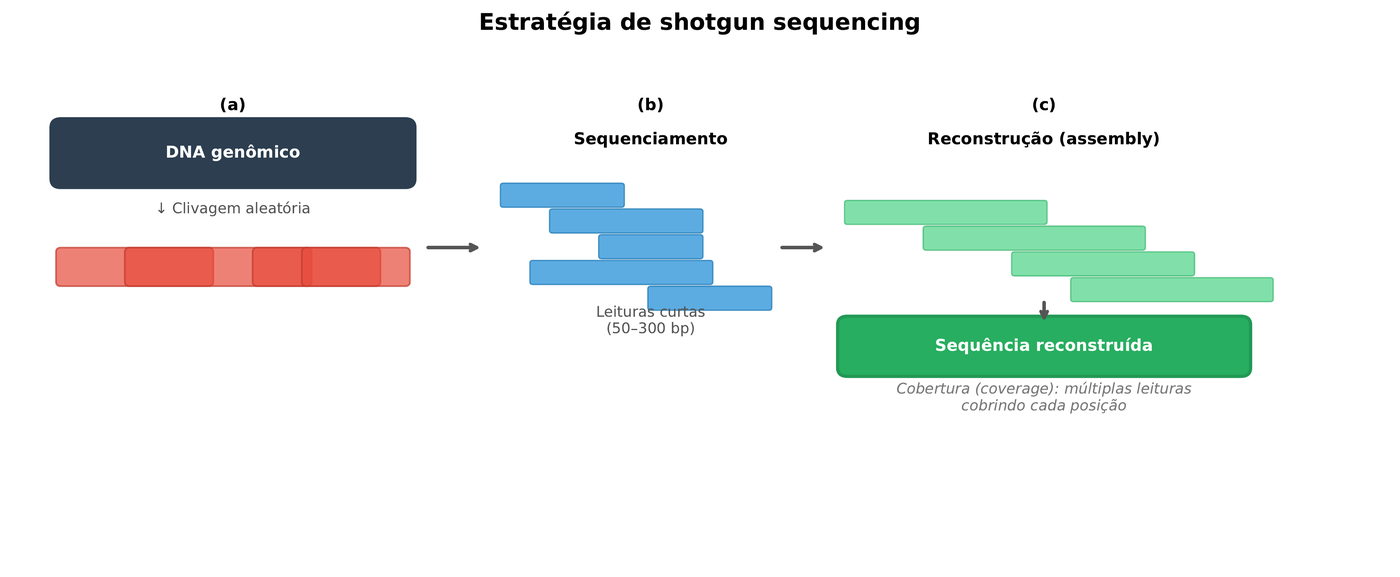
\includegraphics[width=0.85\textwidth]{imagens/shotgun_sequencing.png}
    \caption{Diagrama ilustrativo do processo de \textit{shotgun sequencing}: clivagem aleatória do DNA genômico em fragmentos, sequenciamento em leituras curtas e sobreposição para reconstrução da sequência original.}
    \label{fig:shotgun}
\end{figure}

Na montagem genômica, fragmentos sobrepostos são inicialmente agrupados em \textbf{contigs} (\textit{contiguous sequences} --- sequências contínuas reconstruídas a partir do alinhamento de leituras sobrepostas, análogas a blocos de texto já montados). Quando existe informação adicional que permite inferir a ordem relativa entre diferentes contigs --- como dados de \textbf{leituras pareadas} (\textit{paired-end reads}: pares de leituras gerados a partir das duas extremidades do mesmo fragmento de DNA, com distância conhecida entre elas) ---, esses podem ser organizados em estruturas mais amplas chamadas \textbf{scaffolds}. Assim, enquanto os contigs representam sequências consolidadas diretamente a partir das leituras, os scaffolds constituem hipóteses mais abrangentes sobre a organização genômica, servindo como passo intermediário até a obtenção de montagens completas e anotadas.

As tecnologias de NGS diferem substancialmente no comprimento das leituras produzidas. Sequenciadores Illumina, por exemplo, geram leituras curtas de alta acurácia (50 a 300 pares de bases), que exigem algoritmos sofisticados para lidar com regiões repetitivas. Em contrapartida, tecnologias como PacBio e Oxford Nanopore produzem leituras longas, que podem alcançar milhares de pares de bases em uma única sequência, favorecendo a continuidade da montagem, ainda que a custos mais elevados e com menor rendimento global \cite{ekblom2014}.

% [SUGESTÃO DE FIGURA]: Tabela comparativa das tecnologias de sequenciamento
\begin{figure}[H]
    \centering
    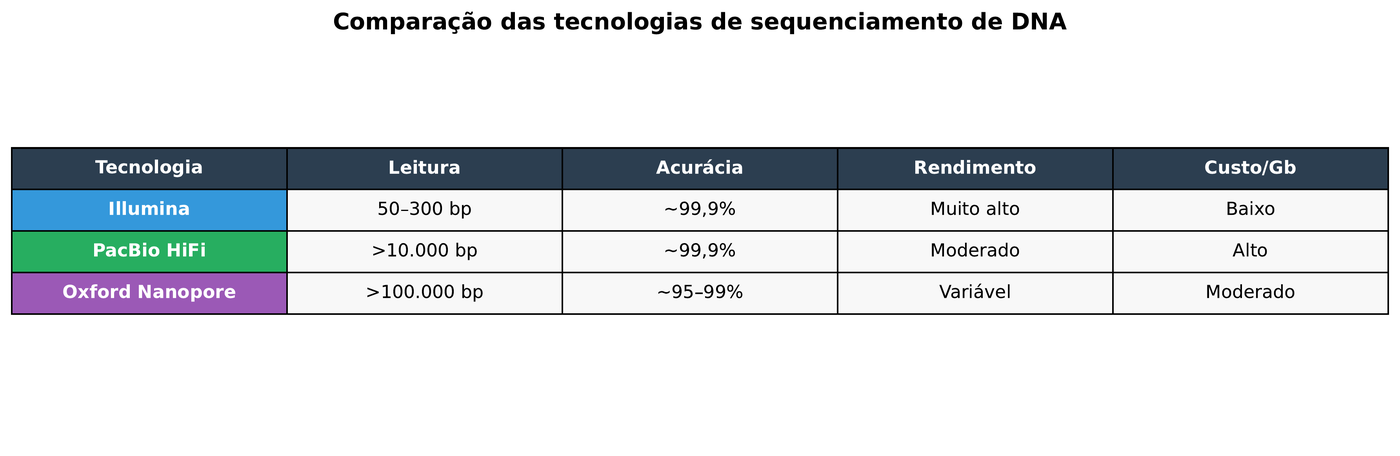
\includegraphics[width=0.85\textwidth]{imagens/tabela_tecnologias_seq.png}
    \caption{Comparativo das principais tecnologias de sequenciamento: Illumina (leituras curtas, alta acurácia), PacBio HiFi (leituras longas, alta fidelidade) e Oxford Nanopore (leituras ultra-longas, menor acurácia).}
    \label{fig:tecnologias_seq}
\end{figure}

O DNA mitocondrial (mtDNA) reúne um conjunto de particularidades que o tornam um alvo privilegiado para a montagem \textit{de novo}. Antes de descrevê-las, convém definir conceitos fundamentais da biologia molecular que serão recorrentes ao longo deste trabalho.

Um \textbf{gene} é um trecho de DNA que contém as instruções para a síntese de uma molécula funcional --- geralmente uma \textbf{proteína}, macromolécula que executa a maioria das funções celulares (catálise enzimática, transporte de substâncias, estrutura celular). O DNA é composto por uma sequência de \textbf{nucleotídeos}, unidades químicas identificadas pelas letras A (adenina), T (timina), G (guanina) e C (citosina). Dois nucleotídeos complementares em fitas opostas (A com T, G com C) formam um \textbf{par de bases} (bp, do inglês \textit{base pair}), a unidade de medida padrão para comprimento de sequências genômicas. A informação genética contida no DNA é lida em blocos de três nucleotídeos consecutivos chamados \textbf{códons}: cada códon especifica um \textbf{aminoácido}, os ``blocos de construção'' das proteínas (existem 20 aminoácidos padrão, como fenilalanina, valina, isoleucina, entre outros). Um gene que codifica uma proteína possui um \textbf{códon de início} (tipicamente ATG, que sinaliza onde a tradução deve começar) e um \textbf{códon de término} ou \textbf{códon de parada} (como TAA, TAG ou TGA, que sinaliza onde a tradução deve parar). O fluxo da informação genética segue o chamado \textbf{dogma central da biologia molecular}: o DNA é transcrito em \textbf{RNA mensageiro} (mRNA), que por sua vez é traduzido em proteína pelos \textbf{ribossomos} --- complexos macromoleculares compostos por proteínas e \textbf{RNA ribossomal} (rRNA). Nesse processo de tradução, cada códon do mRNA é reconhecido por uma molécula de \textbf{RNA transportador} (tRNA), que carrega o aminoácido correspondente e o posiciona no ribossomo para ser incorporado à cadeia proteica em crescimento. A região do tRNA que reconhece o códon é chamada \textbf{anticódon} --- uma sequência de três nucleotídeos complementar ao códon do mRNA \cite{alberts2022}.

Em metazoários (animais multicelulares), o mtDNA corresponde a uma molécula \textbf{circular} de fita dupla --- diferentemente dos \textbf{cromossomos} nucleares (estruturas lineares de DNA compactado localizadas no núcleo da célula, que carregam a maior parte da informação genética), que são lineares, o DNA mitocondrial forma um anel contínuo sem extremidades ---, com tamanho geralmente entre 12 e 22 mil pares de bases, codificando 37 genes distribuídos em 13 proteínas associadas à \textbf{fosforilação oxidativa} (o conjunto de reações bioquímicas que a mitocôndria utiliza para produzir ATP, a molécula de energia da célula), 22 tRNAs e 2 rRNAs \cite{anderson1981,asakawa1995,boore1999}. Em sua revisão seminal, \citeonline{boore1999} observou que, embora a economia extrema de tamanho seja aparente em muitos casos, essa visão --- até então quase axiomática --- é refutada por mitogenomas com grandes quantidades de sequência não codificante descobertos em alguns artrópodes, moluscos e nematódeos, demonstrando que as pressões seletivas sobre o tamanho do mtDNA variam substancialmente entre linhagens. O sequenciamento completo do genoma mitocondrial humano por \citeonline{anderson1981} representou um marco histórico, estabelecendo o modelo de referência para a organização gênica mitocondrial dos metazoários.

% [SUGESTÃO DE FIGURA]: Representação circular de um genoma mitocondrial típico
\begin{figure}[H]
    \centering
    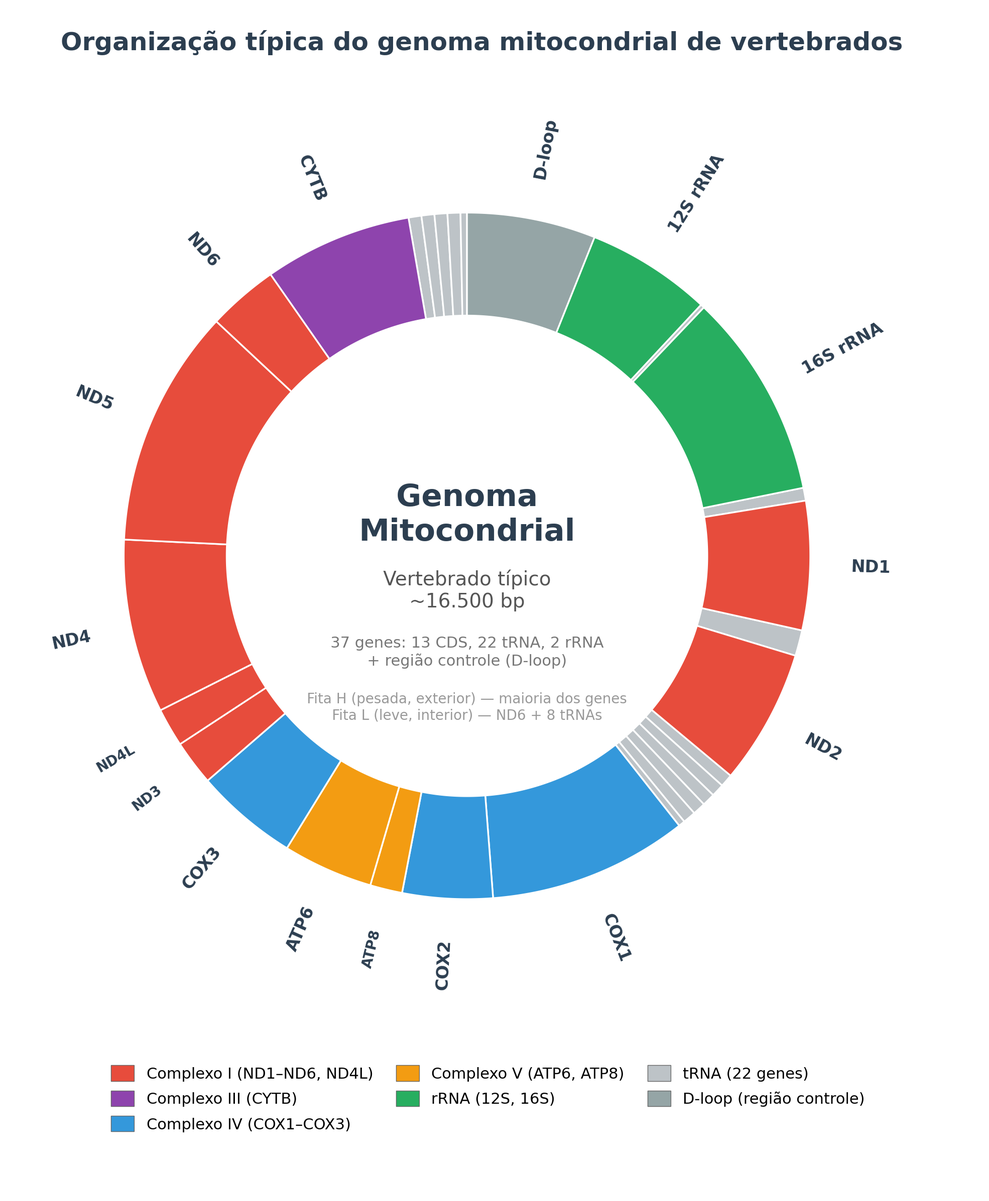
\includegraphics[width=0.75\textwidth]{imagens/mitogenoma_vertebrado_esquematico.png}
    \caption{Representação circular esquemática de um genoma mitocondrial típico de vertebrado, mostrando a distribuição dos 37 genes (13 CDS, 22 tRNAs, 2 rRNAs), a região controle (D-loop) e as fitas pesada (H) e leve (L).}
    \label{fig:mitogenoma_esquematico}
\end{figure}

A ausência de \textbf{íntrons} (segmentos não codificantes que, nos genes nucleares, intercalam as regiões codificantes e precisam ser removidos antes da tradução), a estrutura compacta e a elevada taxa de cópias por célula tornam o mtDNA especialmente acessível, facilitando sua recuperação mesmo em experimentos voltados ao genoma nuclear, nos quais ele aparece como subproduto. Além disso, características funcionais como a herança predominantemente materna, a ausência geral de recombinação e a taxa evolutiva superior à do DNA nuclear ampliam sua utilidade em estudos biológicos. Essas propriedades explicam sua ampla aplicação em análises de genética de populações, \textbf{filogeografia} (estudo da distribuição geográfica de linhagens genéticas), sistemática e conservação da biodiversidade.

Para explorar essas vantagens, foram desenvolvidos algoritmos específicos de montagem. Uma das abordagens mais empregadas é a \textit{seed-and-extend} (semente-e-extensão), em que uma sequência inicial conhecida (\textit{seed} --- semente) --- que pode ser um gene ou até mesmo um fragmento de organela de espécie próxima --- serve como ponto de partida para estender iterativamente a montagem até que a molécula circular seja reconstruída. Quando as extremidades da sequência em construção se sobrepõem, confirmando que o genoma forma um anel contínuo, diz-se que a montagem foi \textbf{circularizada} --- indicação de que o genoma mitocondrial completo foi recuperado com sucesso. O NOVOPlasty é um dos principais programas baseados nessa estratégia, destacando-se pela eficiência na recuperação de genomas mitocondriais e cloroplastidiais a partir de dados de genoma total \cite{dierckxsens2017}. Avanços recentes, como o pipeline MitoHiFi, exploram leituras longas de alta fidelidade, evidenciando a constante evolução das ferramentas voltadas à montagem de organelas \cite{ulianosilva2023}.

% [SUGESTÃO DE FIGURA]: Diagrama da estratégia seed-and-extend
\begin{figure}[H]
    \centering
    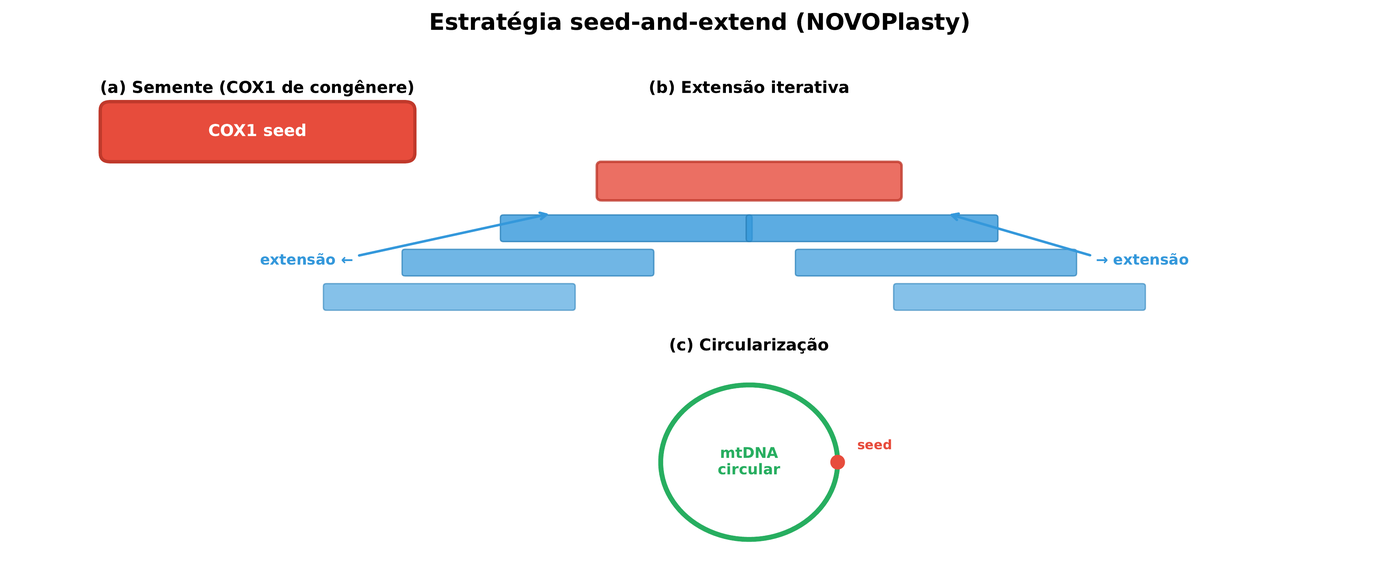
\includegraphics[width=0.85\textwidth]{imagens/seed_and_extend.png}
    \caption{Diagrama ilustrativo da estratégia \textit{seed-and-extend}: (a) sequência semente; (b) extensão iterativa a partir de leituras sobrepostas; (c) circularização quando as extremidades se encontram.}
    \label{fig:seed_extend}
\end{figure}

Complementarmente à montagem, a \textbf{anotação funcional} dos genes mitocondriais permite identificar e classificar os elementos codificantes da molécula reconstruída --- ou seja, determinar quais genes estão presentes, suas posições exatas e suas funções biológicas. Para metazoários, ferramentas como o MITOS2 combinam alinhamentos de homologia (comparações com genes conhecidos em bancos de dados) com modelos de covariância (Infernal) para predizer genes codificadores de proteínas, tRNAs e rRNAs, produzindo anotações em formatos padronizados como \textbf{GFF3} (\textit{General Feature Format version 3} --- formato tabular que especifica a localização e o tipo de cada gene no genoma) \cite{donath2019}. A integração da etapa de anotação em pipelines automatizados de montagem permanece, contudo, uma lacuna na maioria das soluções disponíveis na literatura. A ampla adoção do MITOS2 pela comunidade científica --- empregado como ferramenta primária de anotação em estudos recentes abrangendo vertebrados \cite{zhan2024,kundu2024}, invertebrados terrestres \cite{shi2024,tao2024} e invertebrados marinhos \cite{wei2024,alboasud2024} --- atesta a confiabilidade de seus resultados e reforça a pertinência de sua integração em fluxos automatizados.

\section{Reprodutibilidade em Ciência Computacional}

A reprodutibilidade é um pilar do método científico, consistindo na capacidade de um pesquisador independente replicar um experimento, com os mesmos materiais e métodos, e obter resultados consistentes. Em pesquisas computacionais, isso se traduz na possibilidade de executar o mesmo código e software sobre os mesmos dados e chegar ao mesmo resultado \cite{peng2011,sandve2013}.

Contudo, a ciência moderna enfrenta o que tem sido amplamente denominado como uma ``crise de reprodutibilidade''. Em uma pesquisa abrangente com 1.576 pesquisadores de diversas áreas, \citeonline{baker2016} revelou que 90\% dos entrevistados reconhecem a existência dessa crise --- sendo que 52\% a consideram significativa e 38\% a classificam como leve. Uma barreira crítica identificada por \citeonline{peng2011} é que, em muitos casos, o código computacional utilizado nas análises simplesmente não está mais disponível: softwares interativos frequentemente não registram as ações dos usuários de forma concreta, e mesmo quando scripts são utilizados, a combinação de múltiplos pacotes raramente é preservada de modo reprodutível. No domínio da bioinformática, essa crise é particularmente acentuada devido à alta complexidade dos pipelines de análise. Um único pipeline pode envolver dezenas de ferramentas de software distintas, cada uma desenvolvida por diferentes grupos, em diferentes linguagens de programação e com um conjunto único e, por vezes, conflitante de dependências de bibliotecas e do próprio sistema operacional. A tarefa de instalar e configurar manualmente esse ecossistema de software para replicar uma análise é extremamente suscetível a erros, uma condição frequentemente descrita como \textit{dependency hell} (inferno de dependências) \cite{gruning2018}.

Pequenas variações na versão de uma ferramenta ou de uma biblioteca subjacente podem levar a resultados drasticamente diferentes, comprometendo a validade e a confiabilidade da pesquisa. Essa barreira técnica não apenas dificulta a verificação dos resultados, mas também impede a reutilização e a adaptação de métodos computacionais, contrariando os princípios FAIR (\textit{Findable, Accessible, Interoperable, and Reusable}), que visam maximizar o valor dos dados e das análises científicas ao enfatizar, em particular, a capacidade de máquinas encontrarem e utilizarem dados automaticamente \cite{sandve2013,wilkinson2016,gruning2018,bes2017}.

% [SUGESTÃO DE FIGURA]: Diagrama comparativo do dependency hell
\begin{figure}[H]
    \centering
    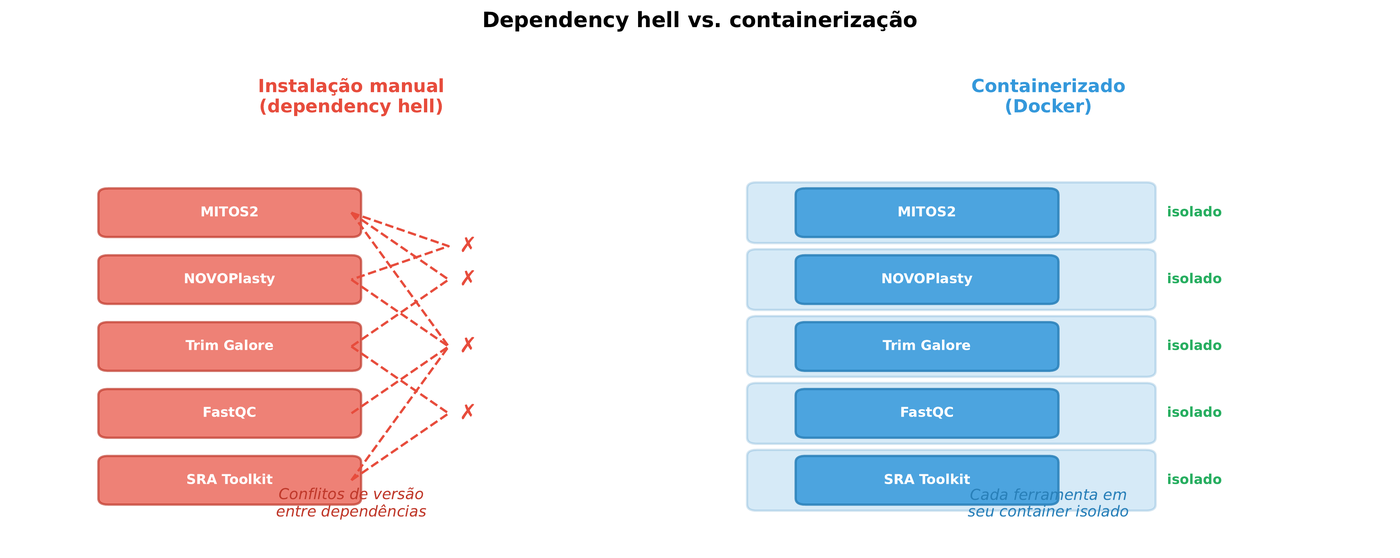
\includegraphics[width=0.85\textwidth]{imagens/dependency_hell.png}
    \caption{Diagrama comparativo do ``inferno de dependências'': à esquerda, instalação manual com conflitos entre versões; à direita, pipeline containerizado com Docker, cada ferramenta em seu container isolado.}
    \label{fig:dependency_hell}
\end{figure}

\section{Tecnologia de Conteinerização com Docker}

Como solução para o problema do \textit{dependency hell} e para garantir a reprodutibilidade computacional, a comunidade científica tem adotado práticas e tecnologias da engenharia de software, com destaque para a virtualização em nível de sistema operacional, também conhecida como containerização. A plataforma Docker se estabeleceu como a principal ferramenta desse paradigma, permitindo o empacotamento de uma aplicação e de todo o seu ambiente de execução --- incluindo bibliotecas, códigos-fonte e dependências --- em uma unidade padronizada e isolada chamada container \cite{merkel2014,gruning2018}.

O funcionamento do Docker baseia-se em dois conceitos centrais: a imagem e o container. A imagem é um template estático e imutável, construído a partir de um arquivo de texto com instruções sequenciais chamado Dockerfile. Esse arquivo serve como uma ``receita'' que define o sistema operacional base, as dependências a serem instaladas e os comandos a serem executados, criando um ambiente de software completo e autocontido. O container, por sua vez, é uma instância executável e isolada de uma imagem. Ao contrário de máquinas virtuais tradicionais, os containers compartilham o kernel do sistema operacional hospedeiro, o que os torna leves e eficientes para iniciar \cite{bes2017}.

Essa arquitetura garante que um software containerizado se comporte de maneira idêntica em qualquer ambiente que possua o Docker instalado --- seja em computadores pessoais, servidores de produção ou ambientes de nuvem --- resolvendo de forma eficaz o problema da inconsistência de ambientes e sendo um passo fundamental para a criação de pipelines científicos portáveis e reprodutíveis \cite{ditommaso2017}.

% [SUGESTÃO DE FIGURA]: Diagrama de camadas da arquitetura Docker
\begin{figure}[H]
    \centering
    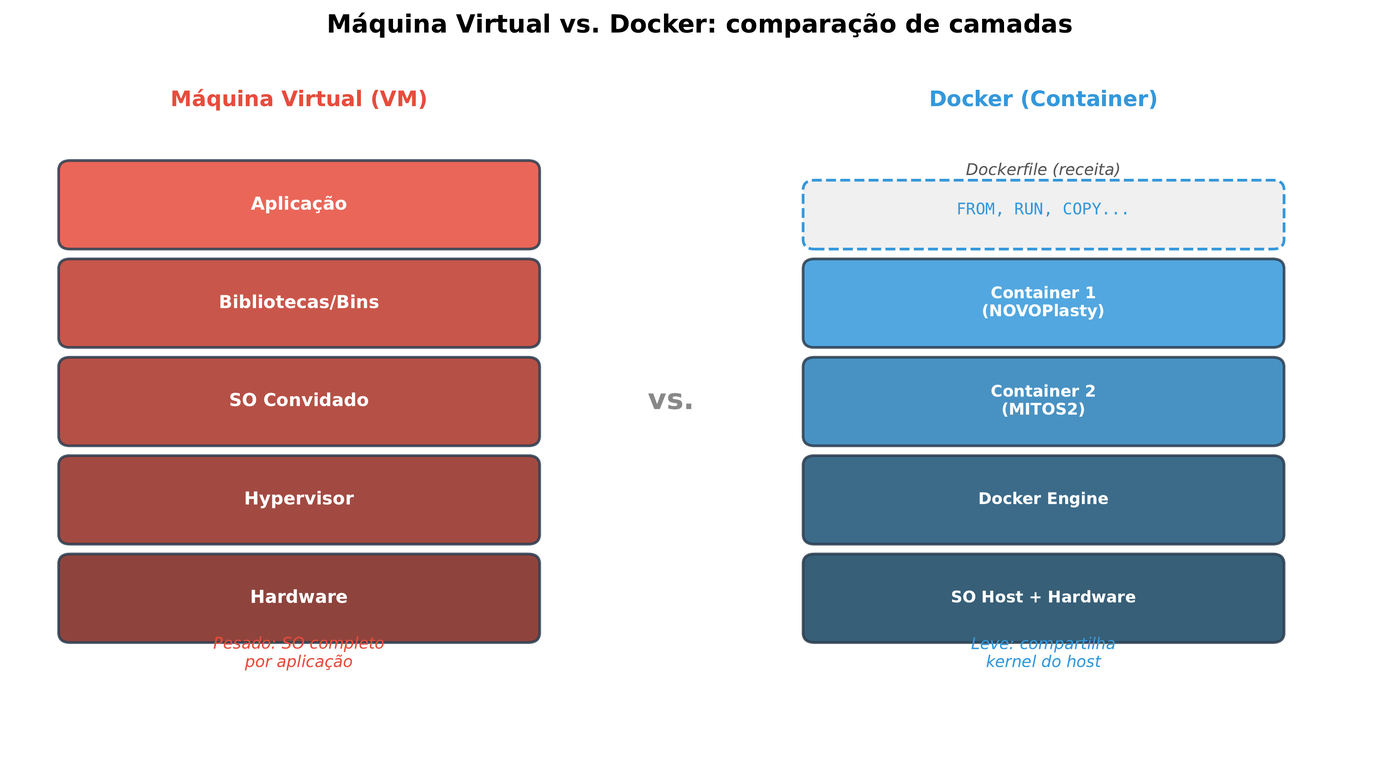
\includegraphics[width=0.85\textwidth]{imagens/docker_vs_vm.png}
    \caption{Comparação entre containers Docker e máquinas virtuais (VM): Dockerfile (receita textual), imagem (template imutável) e container (instância em execução), evidenciando a leveza dos containers.}
    \label{fig:docker_vs_vm}
\end{figure}

\section{Sistemas de Gerenciamento de Workflows Científicos}

A containerização resolve a questão do ambiente de software, mas não a orquestração das múltiplas etapas que compõem uma análise bioinformática. A execução manual e sequencial de cada container é ineficiente e propensa a erros. Para gerenciar essa complexidade, foram desenvolvidos Sistemas de Gerenciamento de Workflows (\textit{Workflow Management Systems}), como o Nextflow \cite{ditommaso2017} e o Snakemake \cite{koster2012}. Essas plataformas permitem que os pesquisadores definam pipelines computacionais complexos por meio de linguagens de alto nível.

Nesses sistemas, um workflow é decomposto em uma série de processos ou regras interconectadas. Cada processo define uma tarefa computacional discreta, especificando seus comandos, suas entradas (arquivos ou variáveis) e suas saídas. O gerenciador de workflow é então responsável por monitorar o estado dos dados e executar os processos na ordem correta, automatizando o fluxo de informação entre as etapas.

A principal vantagem dessas ferramentas reside na abstração da camada de execução. Elas integram-se nativamente com tecnologias como Docker, permitindo que cada processo seja executado em seu próprio container pré-configurado. Além disso, são compatíveis com diversos ambientes de execução, desde computadores pessoais até clusters de computação de alto desempenho (HPC) e plataformas de nuvem. Isso confere ao pipeline características essenciais para a ciência moderna: portabilidade, escalabilidade e retomada automática (\textit{resumability}) em caso de falhas, evitando o reprocessamento de etapas já concluídas.

A combinação de um gerenciador de workflows com a containerização é hoje considerada o padrão-ouro para o desenvolvimento de pipelines de bioinformática, sendo a base de iniciativas comunitárias como o nf-core, que busca padronizar e compartilhar pipelines que seguem as melhores práticas de reprodutibilidade \cite{ewels2020}.

O referencial teórico expôs os conceitos fundamentais que dão suporte à proposta deste trabalho, abordando desde os princípios de montagem \textit{de novo} de genomas até as soluções contemporâneas de reprodutibilidade, como a containerização e os sistemas de gerenciamento de workflows. Esses conceitos fornecem a base conceitual sobre a qual se apoiam os trabalhos relacionados, discutidos no Capítulo~\ref{cap:trabalhos}, que permitem situar a presente proposta no estado da arte da bioinformática aplicada à montagem de mitogenomas.
